% options:
% thesis=B bachelor's thesis
% thesis=M master's thesis
% czech thesis in Czech language
% english thesis in English language
% hidelinks remove colour boxes around hyperlinks

\documentclass[thesis=M,english,hidelinks]{FITthesis}[2012/10/20]

\usepackage[utf8]{inputenc} % LaTeX source encoded as UTF-8
\usepackage{dirtree} %directory tree visualisation
\usepackage{graphicx} %graphics files inclusion
% \usepackage{subfig} %subfigures
% \usepackage{amsmath} %advanced maths
% \usepackage{amssymb} %additional math symbols
\usepackage{todonotes}
\usepackage[acronym,nonumberlist,toc,numberedsection=autolabel,nopostdot]{glossaries}

% % % % % % % % % % % % % % % % % % % % % % % % % % % % % % 
% FORMAL STUFF
% % % % % % % % % % % % % % % % % % % % % % % % % % % % % % 
\department{Department of Software Engineering}
\title{Applying the Normalized Systems Theory on Microservice Architecture}
\authorGN{Vincenc} %author's given name/names
\authorFN{Kolařík} %author's surname
\author{Vincenc Kolařík} %author's name without academic degrees
\authorWithDegrees{Bc. Vincenc Kolařík} %author's name with academic degrees
\supervisor{Ing. Robert Pergl, Ph.D.}
\placeForDeclarationOfAuthenticity{Prague}
\declarationOfAuthenticityOption{1} %select as appropriate, according to the desired license (integer 1-6)

% % % % % % % % % % % % % % % % % % % % % % % % % % % % % % 
% ABSTRACT & KEYWORDS
% % % % % % % % % % % % % % % % % % % % % % % % % % % % % % 

\acknowledgements{THANKS (remove entirely in case you do not with to thank anyone)}
\abstractEN{Summarize the contents and contribution of your work in a few sentences in English language.}
\abstractCS{V n{\v e}kolika v{\v e}t{\' a}ch shr{\v n}te obsah a p{\v r}{\' i}nos t{\' e}to pr{\' a}ce v {\v c}esk{\' e}m jazyce.}

\keywordsCS{Replace with comma-separated list of keywords in Czech.}
\keywordsEN{Replace with comma-separated list of keywords in English.}

% % % % % % % % % % % % % % % % % % % % % % % % % % % % % % 
% ACRONYMS
% % % % % % % % % % % % % % % % % % % % % % % % % % % % % % 
\makeglossaries
\newacronym{CVUT}{{\v C}VUT}{{\v C}esk{\' e} vysok{\' e} u{\v c}en{\' i} technick{\' e} v Praze}
\newacronym{FIT}{FIT}{Fakulta informa{\v c}n{\' i}ch technologi{\' i}}

\newacronym{API}{API}{application programming interface}
\newacronym{AWS}{AWS}{Amazon Web Services}
\newacronym{BE}{BE}{back-end}
\newacronym{EA}{EA}{enterprise architecture}
\newacronym{FE}{FE}{front-end}
\newacronym{IOT}{IoT}{internet of things}
\newacronym{IT}{IT}{information technology}
\newacronym{MAPE}{MAPE}{monitoring, analysis, planning, execution}
\newacronym{MSA}{MSA}{microservice architecture}
\newacronym{MS}{MS}{microservice}
\newacronym{MVC}{MVC}{Model-View-Controller architecture}
\newacronym{MVVM}{MVVM}{Model-View-ViewModel architecture}
\newacronym{NS}{NS}{Normalized Systems theory}
\newacronym{OOP}{OOP}{object oriented programming}
\newacronym{POJO}{POJO}{plain old Java object}
\newacronym{REST}{REST}{representational state transfer}
\newacronym{RPC}{RPC}{remote procedure call}
\newacronym{SA}{SA}{software architecture}
\newacronym{SOA}{SOA}{service-oriented architecture}
\newacronym{SW}{SW}{software}

%%%%%%%%%%%%%%%%%%%%%%%%%%%%%%%%%%%%%%%%%%%%%%%%%%%%%%%%%%%%
%%%%%%%%%%%%%%%%%%%%%%%%%%%%%%%%%%%%%%%%%%%%%%%%%%%%%%%%%%%%
%%                                                        %%
%%                      THE DOCUMENT                      %%
%%                                                        %%
%%%%%%%%%%%%%%%%%%%%%%%%%%%%%%%%%%%%%%%%%%%%%%%%%%%%%%%%%%%%
%%%%%%%%%%%%%%%%%%%%%%%%%%%%%%%%%%%%%%%%%%%%%%%%%%%%%%%%%%%%
\begin{document}

% % % % % % % % % % % % % % % % % % % % % % % % % % % % % % 
% 
% INTRODUCTION
% 
% % % % % % % % % % % % % % % % % % % % % % % % % % % % % % 
\setsecnumdepth{part}
\chapter{Introduction}
\todo[inline,size=\Large]{Missing whole chapter}
\begin{verbatim}
motivace

- same goals, different approach
- microservices = craftmanship
- NS theory of systems
- distributed 


- modularity, granularity, evolvability
- evolvability, adaptation to change
    
    
    
\end{verbatim}

Widely used throughout the industry by leading companies \cite{ms-who-is-using}.

\setsecnumdepth{all}

% % % % % % % % % % % % % % % % % % % % % % % % % % % % % % 
% 
% GOALS AND APPROACH
% 
% % % % % % % % % % % % % % % % % % % % % % % % % % % % % % 
\chapter{Goals and Approach}
\section{Goals}
According to~a~thesis assignment the~following goals were set:
\begin{itemize}
	\item Analyze the current state-of-the-art design methods and industrial applications of microservice architecture.
	\item Identify key features and the most significant challenges encountered in~the~industry.
	\item Discuss compliance of the currently used methods with \acrlong{NS} and explore possibilities for improvements using \acrshort{NS}. 
	\item Formulate guidelines for designing microservices based on the results from the previous chapter, discuss them and demonstrate them on~a~case study if reasonable.
\end{itemize}

\section{Approach}
Microservices architecture is an \acrfull{EA} pattern. \acrshort{EA} could be analyzed in enormously broad context, spanning from business-IT alignment, through \acrshort{SW} development methodologies to a choice of programming languages. This section discusses boundaries for this thesis to make the topic reasonably narrow without overlooking the quintessence of \acrlong{MSA}.

\subsection{Organizational Aspects}
Microservices are often valued for their positive effects on organizations and teams of engineers creating them. Development of end-to-end features and operational responsibility fosters DevOps culture \cite{devops-what-is}. Code ownership and cross-functional teams cultivate team spirit and nurture motivation of developers \cite{ms-fow-new-term-def, ms-modelling-with-petter, ms-building-ms}.

There's also a sociological observation called \textit{Conway's law} that states:
\begin{quote}
    Any organization that designs a system (defined broadly) will produce a design whose structure is a copy of the organization's communication structure.~\cite{conways-law}
\end{quote}

The bi-directional influence between software architecture and the organization that creates it is a remarkable topic, and it would be unwise to ignore it while running a business. Despite that, it will be ignored in this thesis, as it would broaden its scope excessively. The \acrshort{NS} literature \cite{ns-recreating, ns-toward-general-theory} has the same attitude and avoids discussion how the organization influences the \acrshort{SW} and vice versa.

\subsection{Performance aspects}
The \acrlong{NS} describes a set of laws which, if applied strictly, guarantee a system to be free from combinatorial effects, i.e., to be indefinitely evolvable. Until now, the industrial \acrlong{SW} projects \cite{ns-it-isnt-different, ns-exploring-defence} are focused on the evolvability of the \acrshort{SW} artifact and doesn't value any other non-functional requirement as much as evolvability.

On the other hand, \acrlong{MS} came into being due to the need for performance and scalability \cite{ms-building-ms, ms-evolutionary-arch}. The evolvability aspect is never more important that those two mentioned. Therefore this thesis will respect this order and will not sacrifice performance and scalability for the sake of evolvability.

\subsection{Libraries, frameworks and other 3rd party technologies}
\begin{verbatim}
    - turbulent times, new frameworks emerging and be abandoned every day
    - https://github.com/mfornos/awesome-microservices not an extensive list of tech, but will suffice
    - don't bother with choosing and comparing particular 3rd party tech, too small detail
    - exctract the principcle and compare that
\end{verbatim}

\subsection{User Interface and }
\begin{verbatim}
    - tons of presentations layers, frontends, desktop apps, mobile apps, watch apps and gadgets 
    - end with external API \ref{sec:ext_api}
\end{verbatim}

\subsection{General Rules}
In an~effort to~make this work conceptually coherent, there were defined essential principles with which this thesis is created:
\begin{enumerate}
    \item Avoid discussion how organization influences the \acrshort{SW} and vice versa.
    \item Do not sacrifice performance and scalability for the sake of evolvability.
    \item When recommending to use an existing technology, extract the principle and recommend that 
\end{enumerate}

\section{Thesis Structure and Tasks}
To fulfill the goals of this thesis the following finer-grain task was defined. The~final structure of~this work is derived from this task list.
\begin{enumerate}
% 	\item Provide an~overview of~utilized theories and concepts (Chapter~\textit{\nameref{sec:theoretical_background}})
% 	\begin{itemize}
% 		\item Introduce key concepts of~\acrlong{NS}
% 		\item Describe the key principles and motivation for \acrlong{MSA}
% 	\end{itemize}

	\item Analyze the \acrlong{MSA} (Chapter \textit{\nameref{sec:msa_analysis}})
	\begin{itemize}
		\item Perform a literature review on \acrshort{MS} and on application of \acrshort{NS} to \acrshort{MS} and/or related architecture styles and patterns
        \item Extract the essential concepts of state-of-the-art design of \acrshort{MS}
		\item Identify key concerns in \acrshort{MS} design and implementation
	\end{itemize}

	\item Examine compliance of \acrlong{MSA} to \acrlong{NS} (Chapter~\textit{\nameref{sec:msa_compliance}})
	\begin{itemize}
		\item Discuss the architectural patterns and principles using \acrlong{NS}
		\item Apply the \textit{Design Theorems for Stable Software} \cite{ns-towards-evolvable} to the essential concepts from previous chapter
	\end{itemize}	

	\item Summarize design guidelines for \acrshort{MSA} (Chapter~\textit{\nameref{sec:guidelines}})
	\begin{itemize}
		\item Provide concise and comprehensive overview of formulated guidelines
		\item Demonstrate guidelines on suitable case study
	\end{itemize}
	
	\item Summarize successes and failures (Chapter~\textit{\nameref{sec:conclusion}})
\end{enumerate}

% % % % % % % % % % % % % % % % % % % % % % % % % % % % % % 
% 
% Theoretical Background
% 
% % % % % % % % % % % % % % % % % % % % % % % % % % % % % % 
\chapter{Theoretical Background}
\label{sec:theoretical_background}

% 
% Introduction to Normalized Systems
% 
\section{Introduction to Normalized Systems}
\acrfull{NS} is a theoretical framework designed to engineer systems (in its broad meaning) to be able to absorb a set of anticipated changes in an infinite period. The ability to absorb changes ---~\textit{evolvability}~--- is the essential property of studied systems. The theory formulates a set of~\textit{rules of evolvability} backed by formal proofs (more in section \ref{sec:evolvability_rules}).

\subsection{Ongoing Research}
The~theory is being developed at the University of~Antwerp, the~department Management Information Systems of~the~faculty Applied Economics. Due to its success, the~authors, Jan Verelst and Herwig Mannaert, have established the~Normalized Systems Institute for further applied research in the \acrshort{SW} industry.

Although the theory originated in a narrow field --- \acrlong{SW} development, it has been generalized and now is being applied to wide range of various disciplines: from business process modeling through legal documents to first thoughts on civil engineering.~\cite{ns-towards-evolvable}

Due to the focus of this thesis, \acrlong{NS} will be explained on the domain of \acrlong{SW} development.

\subsection{Essential Principles}
\label{sec:evolvability_rules}

\begin{figure}[t]
  \centering
    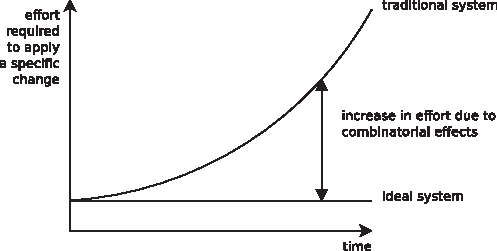
\includegraphics{images/Combinatorial_effects_explained.pdf}
   	\caption{Combinatorial effects explained}
    \label{fig:combinatorial_effects}
\end{figure}

The authors of \acrlong{NS} state the contemporary \acrshort{IT} problems are manifestations of~fundamental flaws in~currently used \acrshort{SW} development methodologies. The Achilles' heel is the evolvability --- adding new features to~existing code base generates \emph{combinatorial effects} (or \textit{instabilities} in newer literature, e.g. \cite{ns-toward-general-theory}), that lead to a~growth of~overall system complexity (see fig. \ref{fig:combinatorial_effects}~\cite{ns-recreating}). Such effects cause to increase the cost of future changes and decrease overall software quality.\cite{ns-recreating}

Initial idea was first uttered by Manny Lehman in~1980:
\begin{quote}
    As an~evolving program is continually changed, its complexity, reflecting deteriorating structure, increases unless work is done to~maintain or reduce it.~\cite{lehman-1980-programs}
\end{quote}

In spite of~that, \acrlong{NS} strive to fulfill the dream articulated by Douglas McIlroy in~1968:
\begin{quote}
    Expect families of~routines to~be constructed on rational principles so that families fit together as building blocks. In short, [the user] should be able safely to~regard components as black boxes.~\cite{mcilroy-1968-mass-software}
\end{quote}

\acrshort{NS} assume that a~change introduced to~a~system is a natural and unavoidable phenomenon. Therefore all rules and principles are designed to~accommodate that fact. The~theory defines a set of~guidelines on how to~engineer the~\acrlong{SW} architecture as a structure of~highly independent modules, which can be added, removed or changed separately. Sufficiently granular architecture will suppress all combinatorial effects during evolution of~the~system.

The~normalized design theorems require a strict separation of~data and actions manipulating that data. Such segregation might be controversial as it contradicts the~essence of~\acrfull{OOP}, which postulates that data and related actions belong into one entity --- a \textit{class}.

% 
% Design Theorems of Stable Software
% 
\section{Design Theorems of Stable Software}
\label{sec:theorems}
This section introduces the four rules of~software evolvability --- \textit{the design theorems of stable software}, which are the building blocks of~\acrshort{NS} theory. An experienced software developer will recognize these rules as they originate from a heuristic design knowledge. The value added by \acrshort{NS} is the theoretical proofs which promote these practical experiences to~defensible theorems. (The proofs are omitted for brevity, but can be found in \cite{ns-recreating, ns-toward-general-theory}.)

\subsection{The Four Theorems}
The \acrshort{NS} theory can prove the system is free from instabilities if and only if the system complies to all the design theorems. Therefore the following postulate is set as an ultimate goal:
\begin{quote}
    An evolving information system should not have \textit{instabilities} (\textit{combinatorial effects}): a bounded amount of additional functional requirements cannot lead to an unbounded amount of additional (versions of) software primitives.~\cite{ns-toward-general-theory}
\end{quote}

\subsubsection{Separation of~Concerns}
\begin{quote}
A processing function can only contain a single task in order to achieve stability.~\cite{ns-toward-general-theory}
\end{quote}

This theorem implies the identification and separation of~every single \textit{task}. Correct separation of~tasks will induce \emph{separation of~concerns} in~the~big picture.

Separation of concerns is a~widely used \emph{best practice} among software architects. However, it is very vaguely formulated. Current manifestations in~software development include for example \emph{multi-tier architectures} (e.g., \acrshort{MVC}, \acrshort{MVVM}) or use of~an~\emph{integration bus} for inter-process communication.

\subsubsection{Data Version Transparency}
\begin{quote}
A structure that is passed through the interface of a processing function needs to exhibit version transparency in order to achieve stability.~\cite{ns-toward-general-theory}
\end{quote}

Data version transparency is an instrument to~cope with an addition or removal a~\emph{data field} in~entity. It implies encapsulation of~the~data fields. Wrapping the~data entity allows co-existence of~various versions of~such entity.

An example from \acrshort{OOP}: data version transparency can be easily achieved by using exclusively the \textit{0-parameter constructor} for instantiation and \emph{accessor methods} for the attribute access (e.g., a \acrshort{POJO}). In that case, all internal data fields are hidden and addition of a new one does not cause processing method to fail.

\subsubsection{Action Version Transparency}
\begin{quote}
A processing function that is called by another processing function, needs to exhibit version transparency in order to achieve stability.~\cite{ns-toward-general-theory}
\end{quote}

Analogously to~previous theorem, various versions of~data entities need to~co-exist in~single system.

This can be achieved by using wrapper functions in procedural programming or by using polymorphism in \acrshort{OOP}.

\subsubsection{Separation of~States}
\begin{quote}
Calling a processing function within another processing function, needs to exhibit state keeping in order to achieve stability.~\cite{ns-toward-general-theory}
\end{quote}

It is a~formalization of~instinctive \emph{avoiding the~transition to an undefined state}. When a~state is kept for every call of a processing function, the~whole system behaves as a~deterministic state machine. This eliminates the~need for complicated recovery from undefined error states.

An example of a~manifestation of~this design theorem is a~database transaction mechanism. The~commit (rollback) action guarantees atomic transition from one defined state to~another.

\subsection{Impacts on Software Development}
The postulate in section \ref{sec:theorems} implies all the \textit{design theorems for stable software} must be consistently followed. The~\acrshort{SW} artifact must be free of~instabilities at compile time, deployment time and run time. It requires the~code base to~be entirely error free, which is not an~easy task to~achieve.

Other inconveniences are inevitably encountered during the development of \acrshort{SW} according to \acrshort{NS}. For example the~\emph{data} and \emph{action version transparency} rules also imply a~lot of~\textit{boilerplate} (non-logic) code (e.g., wrapper classes, accessor methods). For a~human programmer writing code complying with \acrshort{NS} is annoying and frustrating.

On the~other hand, \acrshort{NS} presents a~set of~\emph{software design patterns} (described in \cite{ns-recreating}) which could be easily produced via code generation. The generated boilerplate code skeleton is then enriched with custom code containing business logic and algorithms. In case the skeleton itself is introduced to a change, the custom code is \textit{harvested} and then \textit{re-injected} back to the fully re-generated skeleton.~\cite{vk-bp}

The code generation approach remedies the developers' disgruntlement for sure. However, it requires the development of sophisticated tooling to get the fully \acrshort{NS}-compliant \acrlong{SW} working. The only known implementation --- the \textit{NSX Expanders}\footnote{https://normalizedsystems.org/tools/} --- is capable of production of remarkably granular, yet still \textit{monolithic} applications.

This thesis is an attempt to broaden the application of \acrlong{NS} to a domain of distributed software architectures.

% 
% Software Architecture
% 
\section{Introduction to Software Architecture}
As time goes by, the size and complexity of a software system grow, the design questions soon grow beyond algorithms and data structures. The new problem of the overall system design emerges.

When the problem is untreated, applications soon become tightly coupled, brittle and increasingly difficult to change. Even experienced team of developers without a vision resort to the prosaic layered architecture pattern also known as the \textit{n-tier architecture}, creating implicit layers by separating source-code modules into packages. A result of this practice often is a collection of poorly organized source code, modules and components lack clear borders, responsibilities, and relationships with each other. This primeval architecture style is mockingly called a \textit{the big ball of mud}~\cite{big-ball-mud}.

\subsection{Formal Definition}
Obviously, the topic of \acrfull{SA} is frequently discussed. There are many conferences organized by respected organizations (e.g., IEEE International Conference on Software Architecture\footnote{http://icsa-conferences.org/}, O'Reilly Software Architecture Conference\footnote{https://conferences.oreilly.com/software-architecture/}), many people bear a job title \textit{Software Architect} or \textit{Solutions Architect}\footnote{https://www.glassdoor.com/}. Despite all that, there are many definitions of \textit{software architecture}, and none of them is considered universal.

For example, the IEEE Computer Society defines software architecture as:
\begin{quote}
    [Software] Architecture is the fundamental organization of a system embodied in its components, their relationships to each other, and to the environment, and the principles guiding its design and evolution.~\cite{std-ieee-arch}
\end{quote}

One of the pioneers of \acrlong{SA}, Len Bass, defines this complex discipline as:
\begin{quote}
    The software architecture of a computing system is the set of structures needed to reason about the system, which comprise software elements, relations among them, and properties of both.~\cite{documenting-sw-arch}
\end{quote}

After introducing these two definitions, the domain of \acrshort{SA} seem to be highly abstract and difficult. It is clear there's a need of an instrument, that will help break down this complex domain. Such an instrument can be the \textit{4+1 View Model of Architecture} featured in the next chapter.

% 
% 4+1 View Model of Architecture
% 
\section{4+1 View Model of Architecture}




\begin{figure}[b]
  \centering
    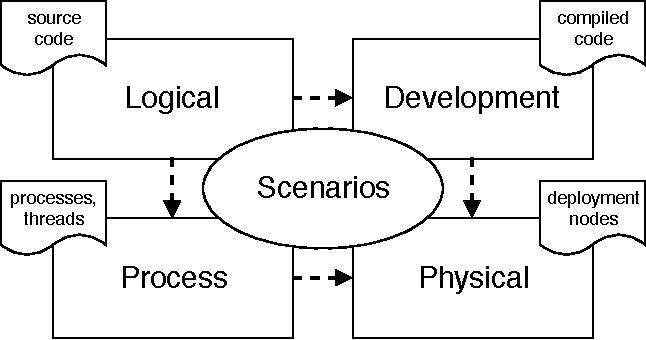
\includegraphics{images/4+1_view.pdf}
    \caption{4+1 View Model of Architecture}
    \label{fig:arch-41-view}
\end{figure}





The “4+1” view model is rather “generic”: other notations and tools can be used, other design methods can
be used, especially for the and the logical and process decompositions, but we have indicated the ones we
have used with succes

THE 4+1 VIEW MODEL OF SOFTWARE ARCHITECTURE
More concretely, an application’s architecture can be viewed from multiple perspec- tives, in the same way that a building’s architecture can be viewed from structural, plumbing, electrical, and other perspectives. Phillip Krutchen wrote a classic paper describing the 4+1 view model of software architecture, “Architectural Blueprints— The ‘4+1’ View Model of Software Architecture” (www.cs.ubc.ca/~gregor/teaching/ papers/4+1view-architecture.pdf). The 4+1 model, shown in Figure 2.1, defines four different views of a software architecture. Each describes a particular aspect of the architecture and consists of a particular set of software elements and relationships between them.
The purpose of each view is as follows:

\begin{itemize}
    \item \textbf{Logical view} covers the The software elements that are created by developers. In object- oriented languages, these elements are classes and packages. The relations between them are the relationships between classes and packages, including inheritance, associations, and depends-on.
    \begin{itemize}
        \item \textbf{Components}: asdf 
    \end{itemize}
    
    \item \textbf{Development view} — The output of the build system. This view consists of mod- ules, which represent packaged code, and components, which are executable or deployable units consisting of one or more modules. In Java, a module is a JAR file, and a component is typically a WAR file or an executable JAR file. The relations between them include dependency relationships between modules and composition relationships between components and modules.
    
    \item \textbf{Process view} components at runtime. Each element is a process, and the relations between processes represent interprocess communication.

    
    \item \textbf{Physical view} How the processes are mapped to machines. The elements in this view consist of (physical or virtual) machines and the processes. The relations between machines represent networking. This view also describes the relation- ship between processes and machines.

\end{itemize}


\section{Architectural Styles}


% % % % % % % % % % % % % % % % % % % % % % % % % % % % % % 
% 
% Microservice Analysis
% 
% % % % % % % % % % % % % % % % % % % % % % % % % % % % % % 

% 
% Design, scope, etc.
% 

\chapter{Analysis of the~Microservice Architecture}
\label{sec:msa_analysis}

\section{(De)composition of Microservice Application}




\textcolor{magenta}{SOA is built on the concept of foster reuse: a share-as-much-as-possible architecture style, whereas microservices architecture is built on the concept of a share-as-little-as- possible style [8]. Given that service reuse has often been less than expected [9], instead of reusing existing microservices for new tasks or use cases, they should be “micro” enough to allow rapidly developing a new one that can coexist, evolve or replace the previous one according to the business needs [10].}





\begin{verbatim}




    - domain dirven design
    - conways's law
    
\end{verbatim}

\subsection{Microservice scope}
microservices are small components, built around business capabilities [3], that are easy to understand, deploy, and scale independently, even using different technology stacks

\begin{verbatim}
    - domain driven development
    - focus on one thing and do it well
        
\end{verbatim}
    One problem with the term microservice is that the first thing you hear is micro. This suggests that a service should be very small. This is also true of other size-based terms such as miniservice or nanoservice. In reality, size isn’t a useful metric.
A much better goal is to define a well-designed service to be a service capable of being developed by a small team with minimal lead time and with minimal collabora- tion with other teams. In theory, a team might only be responsible for a single service, so that service is by no means micro. Conversely, if a service requires a large team or takes a long time to test, it probably makes sense to split the team and the service. Or if you constantly need to change a service because of changes to other services or if it’s triggering changes in other services, that’s a sign that it’s not loosely coupled. You might even have built a distributed monolith.
The microservice architecture structures an application as a set of small, loosely coupled services. As a result, it improves the development time attributes—main- tainability, testability, deployability, and so on—and enables an organization to develop better software faster. It also improves an application’s scalability, although that’s not the main goal. To develop a microservice architecture for your application, you need to identify the services and determine how they collaborate. Let’s look at how to do that.

\subsection{Strong Module Boundaries}

\subsection{Inner vs. Outer Architecture}
\begin{verbatim}
    - focus on outer arch
    - inner - two arguments - it's sth. that can be rewritten by a team in two weeks
    - mention other definition
\end{verbatim}
\begin{figure}
 \missingfigure{\nameref{fig:in-vs-out-arch}}
 \caption{Inner vs. Outer Architecture}
 \label{fig:in-vs-out-arch}
\end{figure}




\subsection{Technological diversity}


\subsection{Tradeoffs of Distributed Architecture}
\subsubsection{Eventual Consistency}
!!!
\subsubsection{Operational Complexity}
\subsubsection{Distribution}




% 
% Communication patterns
% 

\section{Inter-microservice Communication}
The microservice architecture is a distributed architecture, so interprocess communication plays a key role.
\begin{verbatim}
    - direct vs. messaging
    - smart endpoints vs. dumb pipes
\end{verbatim}

\subsection{Interaction Models}
Interaction Models refers to the communication flow among components. Possible values: synchronous, asynchronous.
3.1.1 Interaction styles
It’s useful to first think about the style of interaction between a service and its clients before selecting an IPC mechanism for a service’s API. Thinking first about the inter- action style will help you focus on the requirements and avoid getting mired in the details of a particular IPC technology. Also, as described in section 3.4, the choice of interaction style impacts the availability of your application. Furthermore, as you’ll see in chapters 9 and 10, it helps you select the appropriate integration testing strategy.
There are a variety of client-service interaction styles. As table 3.1 shows, they can be categorized in two dimensions. The first dimension is whether the interaction is one-to-one or one-to-many:
- One-to-one—Each client request is processed by exactly one service
- One-to-many—Each request is processed by multiple services.
The second dimension is whether the interaction is synchronous or asynchronous:
Synchronous—The client expects a timely response from the service and might even block while it waits.
Asynchronous—The client doesn’t block, and the response, if any, isn’t necessar- ily sent immediately.
Table 3.1 The various interaction styles can be characterized in two dimensions: one-to-one vs one-to- many and synchronous vs asynchronous.
Synchronous —
Asynchronous Publish/subscribe Publish/async responses
The following are the different types of one-to-one interactions:
Request/response—A service client makes a request to a service and waits for a response. The client expects the response to arrive in a timely fashion. It might event block while waiting. This is an interaction style that generally results in services being tightly coupled.
Asynchronous request/response—A service client sends a request to a service, which replies asynchronously. The client doesn’t block while waiting, because the ser- vice might not send the response for a long time.



\subsection{Service Interfaces}
\textcolor{magenta}{Service Interfaces are the different means of specifying contracts (if any) for the communication of microservices [45]. Possible values: formal (defined through a formal contract), tech-tied (the interface is tied to the implemen- tation technology), ad-hoc (defined in a novel language).}


\subsection{Data Exchange Protocol}
Data Exchange are the protocols used to represent the communication. Possible values: REST/HTTP, RPC-alike, message queues, other.

% 
% Persistence
% 
\section{Persistence}

\textcolor{magenta}{Eventual Consistency: Maintaining strong consistency is extremely difficult for a distributed system, which means everyone has to manage eventual consistency.}

\textcolor{magenta}{Data Storage usually integrated multiple services in legacy systems, but in microservices architectures it is mandatory to find seams in the databases and use the right technologies to split them out cleanly \cite{ms-building-ms}. Possible values: SQL, graph-oriented, document-oriented, other.}

- one DB per MS pattern 

One key challenge when using messaging is atomically updating the database and publishing a message. A good solution is to use the Transactional outbox pattern and first write the message to the database as part of the database trans- action. A separate process then retrieves the message from the database using either the Polling publisher pattern or the Transaction log tailing pattern and publishes it to the message broker.

% 
% Transaction management
% 
\section{Transaction management}
\label{sec:transaction_management}
After that I look at the two different ways of coordinating sagas: choreography, where participants exchange events without a centralized point of con- trol, and orchestration, 

\subsection{Two-Phase Commit}
\subsection{Three-Phase Commit}
\subsection{The Saga Pattern}


\section{Deployment \& Operations}
\textcolor{magenta}{Independent Deployment: Simple services are easier to deploy, and since they are autonomous, are less likely to cause system failures when they go wrong.}

\textcolor{magenta}{Deployment encompasses how and where services are actually hosted and deployed. Although the cloud has been adopted as the de-facto platform for microservices [44], there are several alternatives into and out of the cloud.}

\textcolor{magenta}{– Platform can be customized due to privacy, security or business constraints. Possible values: public cloud, private cloud, in-house.}

\textcolor{magenta}{– Management encompasses the responsive reaction to failures and changing environmental conditions, minimizing human intervention [7]. Possible val- ues: built-in cloud services (e.g., AWS Cloudwatch and Autoscaling), third- party services (e.g., Rightscale, New Relic), ad-hoc solutions (i.e., tied to the particular approach).}

\subsection{Scalability / Elasticity}
\label{sec:scalability}
– Scalability and elasticity refer to the capability to rapidly adjust the overall capacity of the platform by adding or removing resources, also minimizing human intervention [7]. Possible values: vendor-provided, autonomic MAPE loops, configuration servers, other.
\subsection{Availability and Resilience}
\textcolor{magenta}{Simply handling both service-level and low-level failures that demand for persistence and recovery techniques [45]. Possible values: resilience patterns, fault injection, error-handling policies, resilience tests, other.}
% 
% External API Design
% 
\section{External API}
\label{sec:ext_api}


\section{Transaction management}


% 
% Cross-cutting concerns
%
\section{Cross-cutting concerns}
\subsection{Security}
\begin{verbatim}
    - Sessions auth
    - JWT/token authentication
\end{verbatim}

\missingfigure{JWT vs. Session authentication call diagram}

\subsection{Observability}
\subsubsection{Monitoring}
\subsubsection{Logging}


% % % % % % % % % % % % % % % % % % % % % % % % % % % % % % 
% 
% Towards stable microservices
% 
% % % % % % % % % % % % % % % % % % % % % % % % % % % % % % 

\chapter{Towards Stable Microservice Architecture}
\label{sec:msa_compliance}
\section{Mapping NS Elements to Microservice Architecture}

\todo[inline,size=\Large]{Missing whole chapter}

\chapter{Guidelines for Stable Microservice Architecture}
\label{sec:guidelines}
\todo[inline,size=\Large]{Missing whole chapter}

% % % % % % % % % % % % % % % % % % % % % % % % % % % % % % 
% 
% Conclusion
% 
% % % % % % % % % % % % % % % % % % % % % % % % % % % % % % 
\setsecnumdepth{part}
\chapter{Conclusion}
\label{sec:conclusion}
\section{Evaluation of Goals}
\todo[inline,size=\Large]{Missing section}

\section{Thoughts on Utilization}
\todo[inline,size=\Large]{Missing section}

\section{Future Work}
\todo[inline,size=\Large]{Missing section}

%%%%%%%%%%%%%%%%%%%%%%%%%%%%%%%%%%%%%%%%%%%%%%%%%%%%%%%%%%%%
%%%%%%%%%%%%%%%%%%%%%%%%%%%%%%%%%%%%%%%%%%%%%%%%%%%%%%%%%%%%
%%                                                        %%
%%                    REFERENCES ETC.                     %%
%%                                                        %%
%%%%%%%%%%%%%%%%%%%%%%%%%%%%%%%%%%%%%%%%%%%%%%%%%%%%%%%%%%%%
%%%%%%%%%%%%%%%%%%%%%%%%%%%%%%%%%%%%%%%%%%%%%%%%%%%%%%%%%%%%

\bibliographystyle{iso690}
\bibliography{DP_references}

\setsecnumdepth{all}
\appendix

\printglossary[type=\acronymtype,toctitle=]

\chapter{Contents of enclosed CD}
\begin{figure}
	\dirtree{%
		.1 readme.txt\DTcomment{the file with CD contents description}.
        .1 Figures\DTcomment{source files of figures used in the thesis}.
        .1 Text\DTcomment{thesis text}.
            .2 DP\_Kolarik\_Vincenc.pdf\DTcomment{PDF version of~the~thesis}.
            .2 src\DTcomment{\LaTeX{} source codes of~the~thesis}.
    }

\end{figure}

\listoftodos

\end{document}